\section{Method}
\label{sec:method}
In this section, we describe the way of how we realized the Moody tool. We present the system architecture and explain how we implement the facial and vocal emotion recognition model in more detail.

\subsection{System Architecture}
\label{subsec:method_system_architecture}
The Moody app is a browser-based application written in TypeScript\footnote{\url{https://www.typescriptlang.org/} (last accessed 07/28/2021)} using the React framework\footnote{\url{https://reactjs.org/} (last accessed: 07/23/2021)}. We make use of the AWS platform for data storage and hosting. In particular, we leverage AWS Amplify which covers the whole software lifecycle of mobile- and web applications from development to continuous deployment (CD) and maintenance\footnote{\url{https://aws.amazon.com/amplify/} (last accessed: 07/23/2021)}. Figure~\ref{fig:system_architecture} depicts the high-level system architecture.

\begin{figure}
\centering
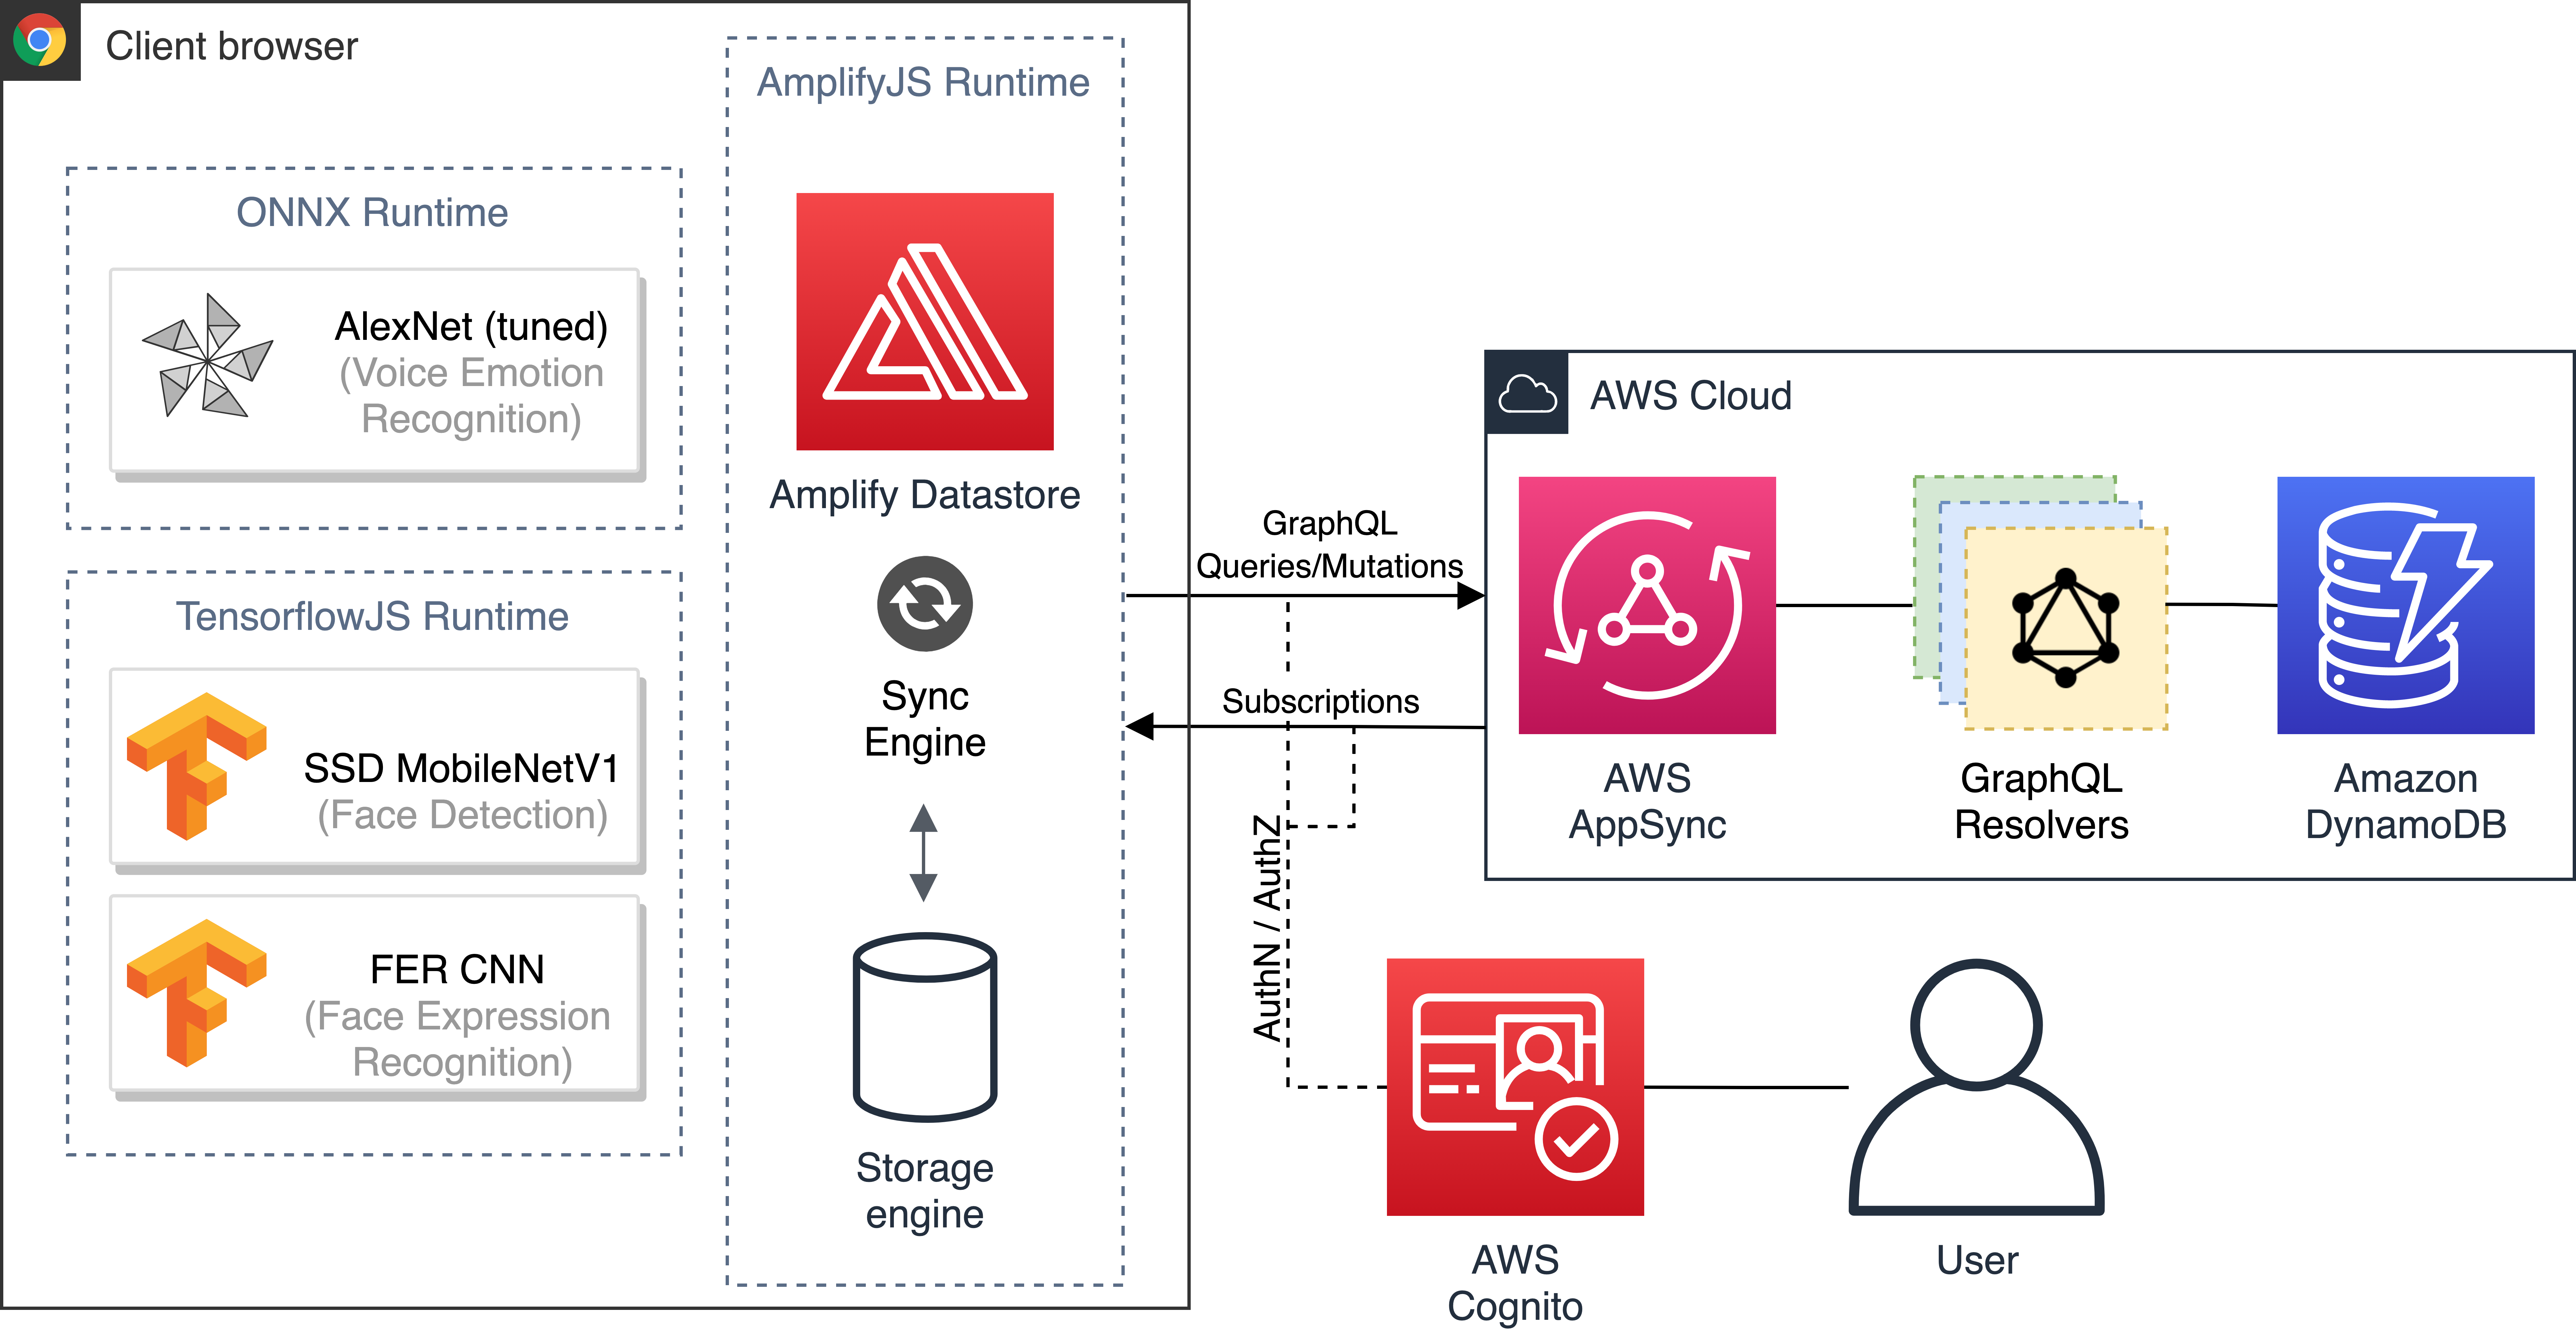
\includegraphics[width=1\textwidth]{assets/system_architecture.png}
\caption{System Architecture Diagram. Moody features a client-server architecture built on top of the AWS platform.}
\label{fig:system_architecture}
\end{figure}

The client-side of the application consists of three major subsystems. The first subsystem is AmplifyJS, which is AWS Amplify's software development kit (SDK) for JavaScript-based applications. For us, it provides the means for data modeling, data persistence across devices as well as user authentication and authorization. Our data is modeled according to the third normal form \cite{codd_further_1972}. The full relational schema can be found in Figure~\ref{fig:erd}, Appendix. Amplify Datastore provides an API to a native storage engine that synchronizes asynchronously with the Cloud in the background\footnote{\url{https://docs.amplify.aws/lib/datastore/getting-started/q/platform/js} (last accessed: 07/23/2021)}. The main advantage of this local first approach is a reactive UI because user interaction is decoupled from the network. We keep the UI state consistent across all components using Redux\footnote{\url{https://redux.js.org/} (last accessed: 07/23/2021)} as a state management tool.

The two other subsystems form the machine learning part of Moody. We decided to run all machine learning algorithms locally in the browser of the user. This is beneficial because the internet connection is not impacted by transferring large image and sound data to a remote server every second. In addition, it supports user privacy as only aggregated emotion scores are saved in the Cloud. One drawback is that slower computers might not handle the inference load very well.

The two face models use the TensorflowJS runtime\footnote{\url{https://www.tensorflow.org/js/} (last accessed: 07/23/2021)} and run in a WebGL context\footnote{\url{https://developer.mozilla.org/en-US/docs/Web/API/WebGL_API} (last accessed: 07/23/2021)} allowing for fast computations of the video stream provided by the user. This video stream is captured using the Screen Capture API\footnote{\url{https://developer.mozilla.org/en-US/docs/Web/API/Screen_Capture_API} (last accessed: 07/23/2021)} implemented by all major browsers. As a presenter, you typically want to select the window where the faces of your audience are located. Moody will then detect bounding boxes for these faces and perform expression prediction every second giving the presenter feedback. Please note that at the time of writing it is not possible to select a specific window to share in Safari.

Our voice emotion model is originally written in Python with the PyTorch framework\footnote{\url{https://pytorch.org/} (last access: 07/23/2021)}. As it is not possible to run Python code efficiently in the browser we leverage ONNX. ONNX is a standardized open-source format to represent neural networks as computation graphs and is currently maintained by the community and Microsoft. It comes along with highly optimized runtimes for different platforms with even better inference performance as compared to the original framework (in our case PyTorch) \cite{onnx_runtime_developers_onnx_2021}. \texttt{onnxruntime-web}\footnote{\url{https://github.com/microsoft/onnxruntime/tree/master/js/web} (last accessed: 07/23/2021)} is the browser runtime which we use to run the voice emotion model. Since the WebGL backend is not yet feature-complete we run our model on the client CPU with WebAssembly\footnote{\url{https://webassembly.org/} (last accessed: 07/23/2021)}. WebAssembly is a compilation target for native languages like C(++) or Rust and allows code execution at close to native speed in the browser. It is currently supported by more than 90\% of all browsers\footnote{\url{https://www.tensorflow.org/js/guide/platform_environment#why_wasm} (last accessed: 07/23/2021)}. To capture the sound of the speaker's microphone we utilize the Web Audio API\footnote{\url{https://developer.mozilla.org/en-US/docs/Web/API/Web_Audio_API} (last accessed: 07/23/2021)}. As a speaker, you are also given the possibility to select the input device. When the voice tracking is active Moody will predict voice emotions every 2.1 seconds and give the speaker live feedback.

All data which is collected from user interaction and the machine learning model predictions is persisted in the AWS Cloud to be available across devices and for further research analysis. Therefore, we have deployed a GraphQL API endpoint with AWS AppSync\footnote{\url{https://aws.amazon.com/appsync/} (last accessed: 07/23/2021)}. This endpoint is called by Amplify Datastore in the background to synchronize new data with the backend. AppSync authorizes each request with AWS Cognito which we use for user authentication. As AppSync is data source agnostic it needs resolvers telling it how to interact with a backend. We chose DynamoDB as the database backend\footnote{\url{https://aws.amazon.com/dynamodb/} (last accessed: 07/23/2021)}. Luckily, Amplify creates these resolvers automatically given a GraphQL compliant data schema\footnote{\url{https://spec.graphql.org/June2018/#sec-Type-System} (last accessed: 07/23/2021)}.

\subsection{Facial Emotion Recognition}
\label{subsec:method_facial_emotion_recognition}
We implement our facial emotion recognition with the \texttt{faceapi.js}\footnote{\url{https://justadudewhohacks.github.io/face-api.js/docs/index.html} (last accessed: 07/23/2021)} JavaScript API for face detection, which is implemented itself on top of the TensorFlowJS core API and can perform face recognition in the browser. To execute in this project both, the face detection itself and the face expression/emotion recognition, we use two neural networks. The input data are single images from the live video conference, which are picked up from the meeting tool (e.g. Zoom) window where the participants' cameras appear. This desktop window has to be selected by the Moody user before he starts the emotion tracking. The two models, which are briefly presented below, were already developed and provided by the authors of \texttt{faceapi.js}, which is why no more data preprocessing was necessary and these only had to be implemented in our system architecture.

First, the algorithm has to detect the faces in the live video and create bounding boxes around the corner points of the faces. For this purpose \texttt{face-api.js} uses the SSD (Single Shot Multibox Detector) MobileNetV1 face detection model\footnote{\url{https://justadudewhohacks.github.io/face-api.js/docs/classes/ssdmobilenetv1.html} (last accessed: 07/30/2021)} \cite{howard_mobilenets_2017}. The neural net will compute the positions of each face in a picture and return the bounding boxes and their occurrence probabilities for each face. Instead of then focusing on short inference time, this face detector aims for high accuracy in recognizing face bounding boxes. Nevertheless, the size of the quantized model is rather small at about 5.4 MB and thus it works at an acceptable speed. This face detection model has been trained on a dataset called 
\emph{WIDERFACE} which was developed by the authors \citeA{yang_wider_2016} and is a face detection benchmark dataset from publicly available images. The authors chose 32,303 images and labeled 393,703 faces on these with a high degree of variability in scale, pose, and occlusion. The weights for the SSD MobileNetV1 model and the final face detector, powered by the TensorFlow object detection API\footnote{\url{https://github.com/tensorflow/models/tree/master/research/object_detection} (last accessed: 07/30/2021)} and trained by \citeA{yang_wider_2016}, were provided by yeephycho\footnote{\url{https://github.com/yeephycho} (last accessed: 07/23/2021)} in a GitHub-Repository\footnote{\url{https://github.com/yeephycho/tensorflow-face-detection} (last accessed: 07/23/2021)}.

The second neural net uses the detected faces and their bounding boxes as an input for the facial expression recognition model. When all faces were detected on an image, the model receives this information and returns an array consisting of all detected faces and their belonging face expressions. The input images in our tool are single frozen frames of the videoconference camera screen. The authors of \texttt{faceapi.js} claim that it is fast and provides reasonable accuracy. The model is about 310 kB in size and uses depthwise separable convolutions as well as densely connected blocks. It was trained on a variety of photos, including photographs scraped from the web and images from publicly available sources. Wearing glasses or low light conditions may reduce the accuracy of the prediction results.

\subsection{Vocal Emotion Recognition}
\label{subsec:method_vocal_emotion_recognition}
In the following sections, we will explain how we preprocess our data regarding our voice emotion model, as well as how we set the model up and train it. We use the datasets introduced in Section~\ref{sec:related_work} as well as a self-designed CNN based on an AlexNet architecture.

\subsubsection{Data Preprocessing}
\label{subsubsec:method_vocal_emotion_recognition_data_preprocessing}
The input we will need later for our voice model is the waveform of the sound which needs to be preprocessed. To avoid fitting the dataset specific volume of the audio samples we apply RMS audio normalization. It is a form of loudness normalization which brings heterogeneous audio sequences to a consistent sound level. We use the formula described by Equation \ref{eq:rms_normalization} for this purpose where $y_n$ is the $n^{th}$ normalized audio sample and $x_n$ the original audio sample in an audio sequence of $N$ samples in total. $r$ is a hyperparameter describing the target RMS level\footnote{\url{https://pydiogment.readthedocs.io/en/latest/_modules/pydiogment/auga.html#normalize} (last accessed: 07/23/2021)}:
\begin{equation}
\label{eq:rms_normalization}
y_n=\sqrt{\frac{N-10\,(\frac{r}{20})}{\sum_{i=0}^{N-1}{x_i^2}}}\cdot{}x_n
\end{equation}
Then the normalized waveform is converted into Mel spectrograms. This step is part of a feature extractor block in the final neural network. We use 128 Mel coefficients. We do this with the \texttt{torchlibrosa} library \cite{kong_panns_2020}. In this library we have re-implemented the Short-Time-Fourier-Transform (STFT) as a CNN with Conv2d layers so that it is compatible with \texttt{onnxruntime-web} \cite{onnx_runtime_developers_onnx_2021}. The STFT is a Fourier Transform version that uses a sliding time window to break up the audio signal into smaller chunks. We use a window size of 2,048 and a sample rate of 22,050. It takes each section of the Fast Fourier Transform (FFT) and then combines them. As a result, it can catch changes in frequency over time \cite{griffin_signal_1984}. To get in the end more data and therefore better training results, we augmented our existing data sets (RAVDESS, TESS, JL-Corpus, EMO-DB) with common data augmentation methods. We used stretching and squeezing (randomly slow down or speed up the sound), background noise (add some random values to the sound), random shifting (shift audio to the left or the right by a random amount), left- and right-trimming (cut off any silence in the beginning or end), and pitch tuning (randomly modify the frequency of parts of the sound)\cite{mcfee_librosa_2015}. The voice emotions are recorded in time windows of 2.1 seconds. This time is the average duration of the samples in the datasets we use.

\subsubsection{AlexNet Architecture}
\label{subsubsec:method_vocal_emotion_recognition_alexnet_architecture}
The input for the voice emotion model is an RMS-normalized sound sequence of length 463,050. In a first feature extractor block, the neural network automatically extracts Mel spectrograms from the sound waveform as described in Section~\ref{subsubsec:method_vocal_emotion_recognition_data_preprocessing}. A major advantage of having the feature extraction as part of the model is that this step does not have to be re-implemented for each programming language -- in our case JavaScript -- thus leading to consistent preprocessing and prediction results independent of the environment.

These Mel spectrograms serve as input for the convolutional neural network part. Based on the datasets introduced in Section~\ref{subsec:related_work_vocal_emotion_recognition} we train the model. We have tried out two well-known architectures: ResNet18 and AlexNet \cite{krizhevsky_imagenet_2012,he_deep_2015}. The performance of both models is very similar, only the size of the models differs. Since the AlexNet with 32.3 MB is almost half the size of the ResNet18 with 59.7 MB and has fewer parameters, we decided to use the AlexNet for our web app (cf. Section~\ref{subsec:results_vocal_emotion_recognition}). This is then exported to ONNX to be executed in the browser with the help of \texttt{onnxruntime-web} for inference.

Additionally, we have modified the default AlexNet architecture with the goal to reduce overfitting by adding batch normalization, layer normalization, and dropout layers. Figure~\ref{fig:alexnet_architecture} illustrates the detailed architecture. Since we use cross-entropy loss\footnote{\url{https://pytorch.org/docs/stable/generated/torch.nn.CrossEntropyLoss.html} (last accessed: 08/02/2021)} as loss function the model output are the raw logits. Applying the softmax function\footnote{\url{https://pytorch.org/docs/stable/generated/torch.nn.functional.softmax.html} (last accessed: 02/08/2021)} on this vector will yield the corresponding class probabilities for each emotion.

\begin{figure}
    \centering
    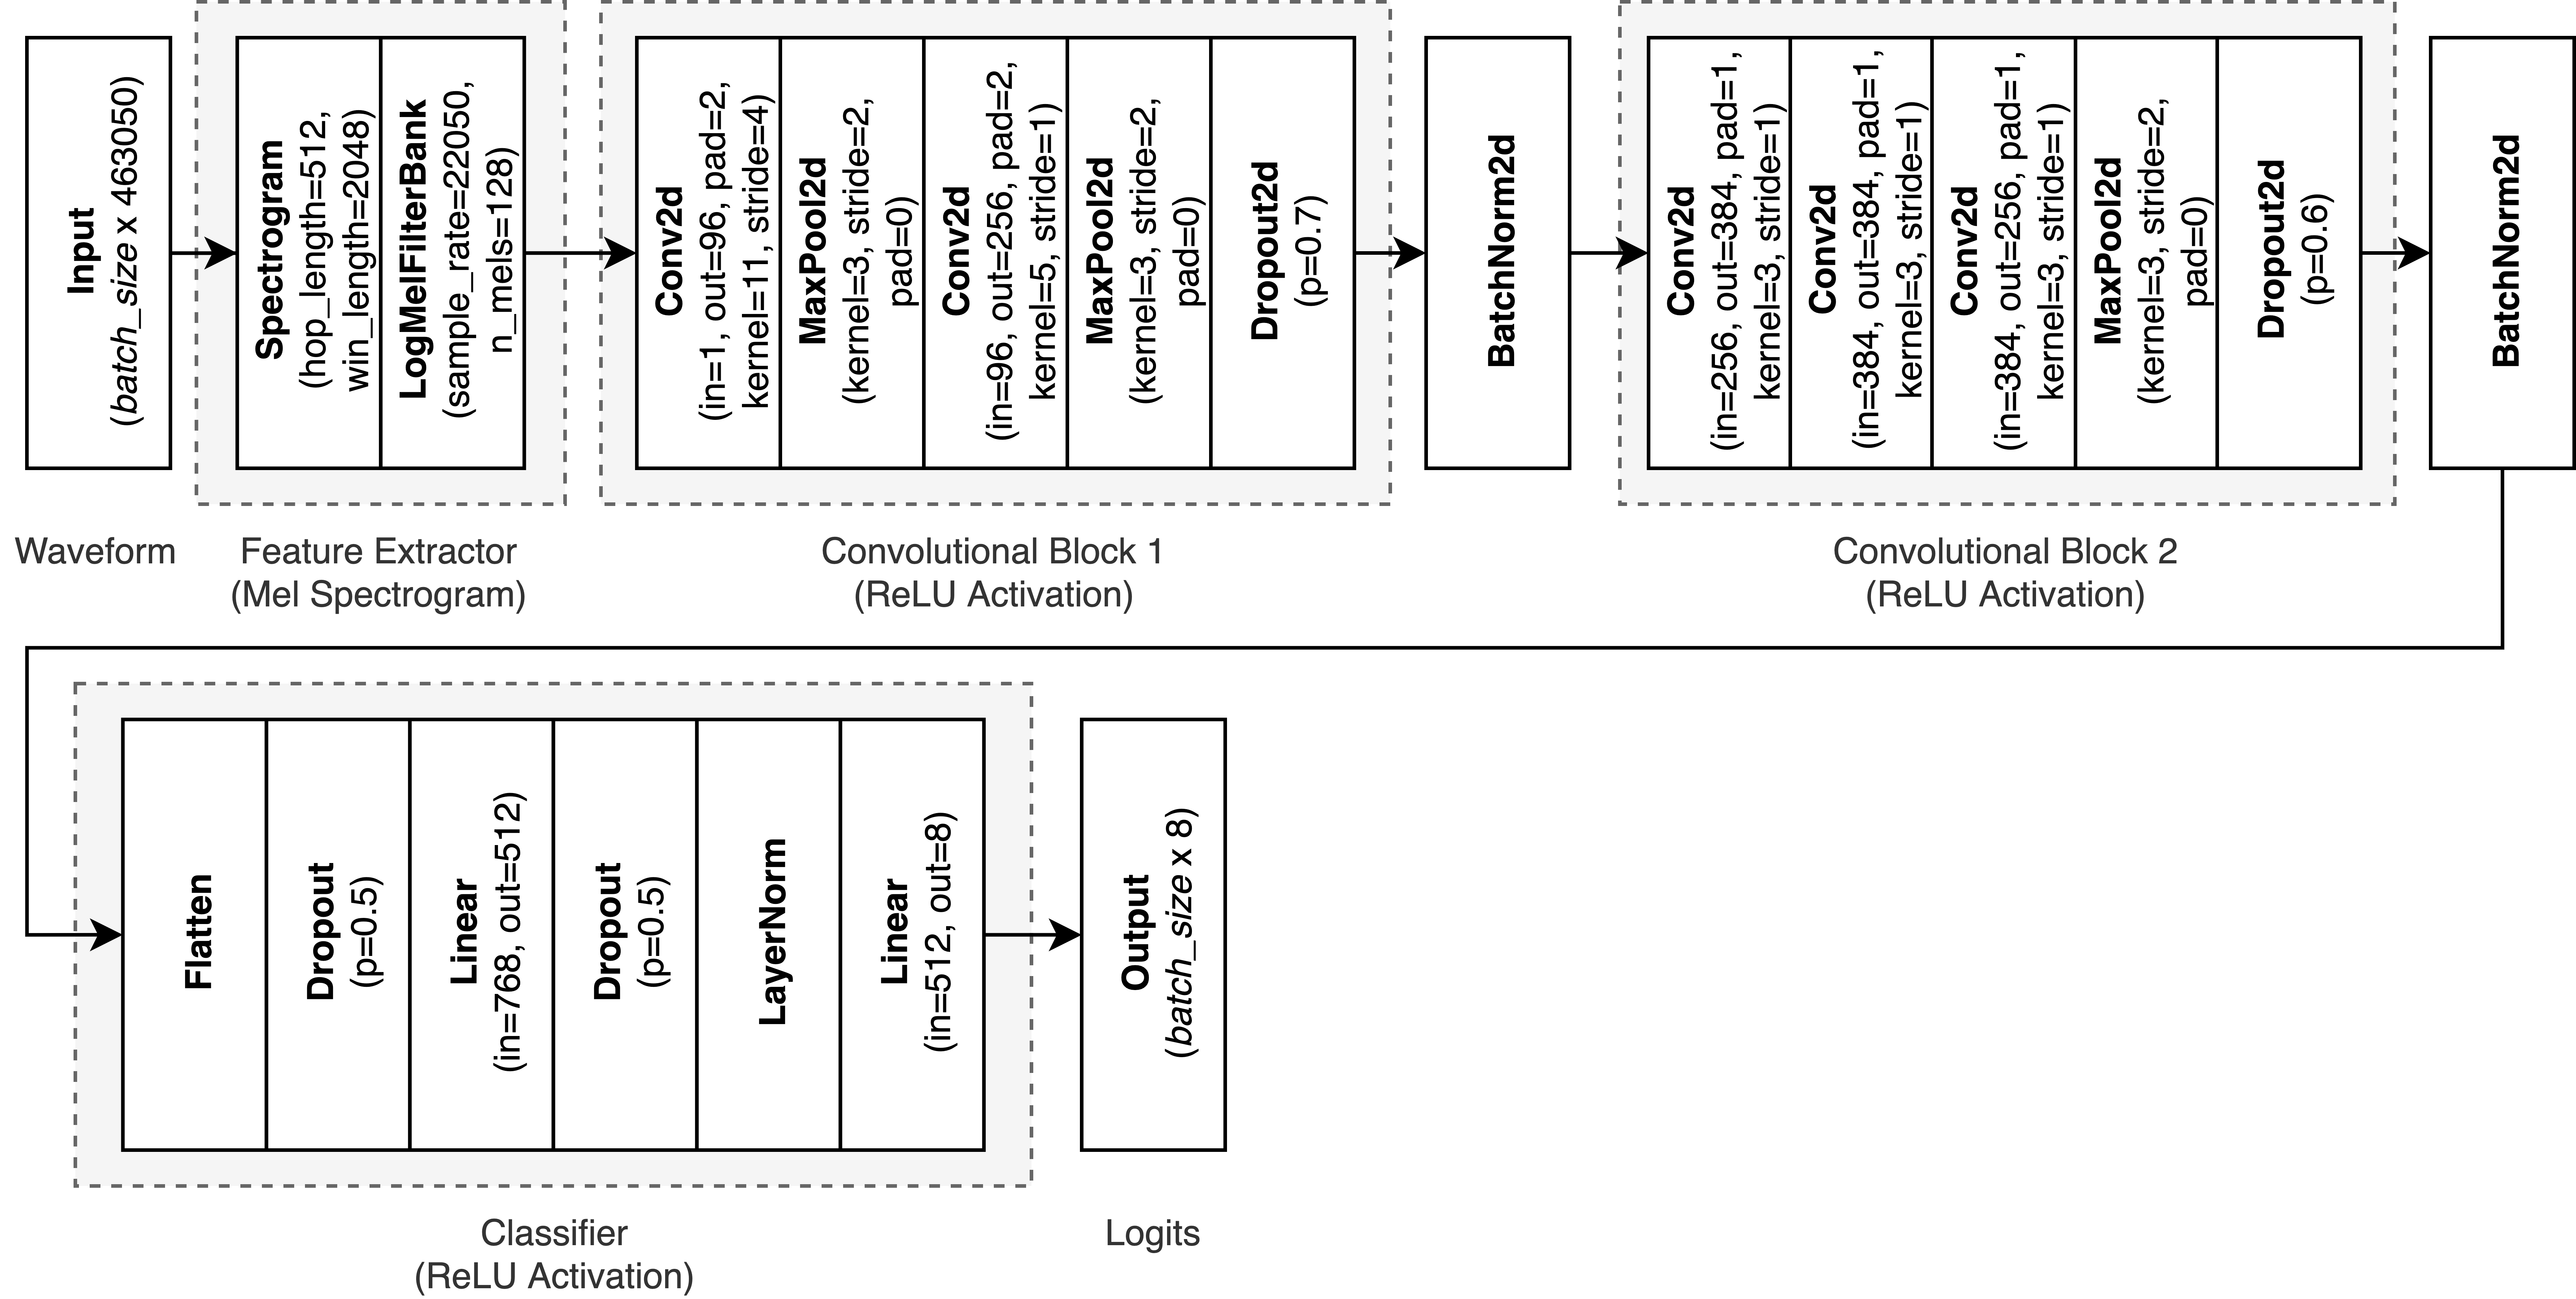
\includegraphics[width=\textwidth]{assets/alexnet_architecture.png}
    \caption{The modified AlexNet architecture of Moody's voice emotion model. All \emph{Conv2d} and \emph{Linear} layers are connected via the ReLU activation function.}
    \label{fig:alexnet_architecture}
\end{figure}
